\documentclass{article}
\usepackage{graphicx} % Required for inserting images
\usepackage{amsmath}
\usepackage{hyperref}
\usepackage{subcaption}

\newcommand{\Lp}{\mathcal{L}}

\title{Automatique TP2}
\author{Alexis Brossier - 12205984}
\date{Mars 2024}

\begin{document}

\maketitle

Les fichiers sources sont disponibles sur \href{https://github.com/AL3X-69/GEP2014L/blob/master/tp2.m}{GitHub}

\section{Étude d'un correcteur proportionnel}
\subsection{}
\begin{figure}[h]
    \centering
    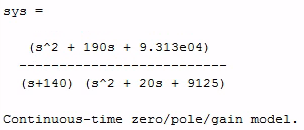
\includegraphics[width=0.5\linewidth]{zpk211.png}
    \caption{Fonction de transfert du système selon MATLAB}
    \label{fig:zpk211}
\end{figure}
\subsection{}
\begin{align*}
    H_0^P(s)&=\frac{N_0(s)}{D_0(s)}=C(s)H(s)=K_C\frac{s^2+190s+93130}{(s+140)(s^2+20s+9125)}\\
    H_e^P(s)&=\frac{D_0(s)}{D_0(s)+N_0(s)}=\frac{(s+140)(s^2+20s+9125)}{K_C(s^2+190s+93130)+(s+140)(s^2+20s+9125)}
\end{align*}
\subsection{}
L'erreur statique est donnée par :
\begin{equation*}
    e_0=\lim_{s\rightarrow0}H_e^P(s)=\frac{140\times9125}{K_C\times93130+140\times9125}=\frac{1277500}{93130\times K_C+1277500}
\end{equation*}
On cherche ensuite $K_C$ tel que $e_0<0.01$, soit :
\begin{gather*}
    e_0<0.01\\
    \frac{1277500}{93130\times K_C+1277500}<0.01\\
    K_C>135.8
\end{gather*}
\subsection{}
\begin{figure}[h]
    \centering
    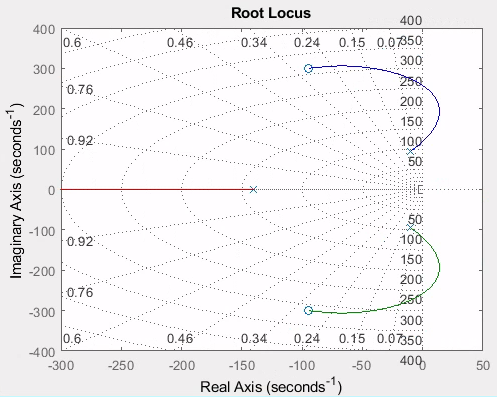
\includegraphics[width=0.75\linewidth]{rlocus214.png}
    \caption{Lieu des poles}
    \label{fig:rlocus214}
\end{figure}
On remarque que les pôles sont stables pour les valeurs de $K_C\in[0;11.2]\cup[267;+\infty[$.
\subsection{}
En relevant les valeurs du diagramme de Nyquist, on peut trouver les comportements asymptotiques suivants :
\begin{equation*}
    \begin{cases}
        \begin{cases}
            \mathcal{R}=0.775\\
            \mathcal{I}=0\\
        \end{cases}&\text{pour }\omega\rightarrow0\\
        \begin{cases}
            \mathcal{R}\rightarrow0^-\\
            \mathcal{I}\rightarrow0^+\\
        \end{cases}&\text{pour }\omega\rightarrow+\infty\\
    \end{cases}
\end{equation*}
\begin{figure}[h]
    \centering
    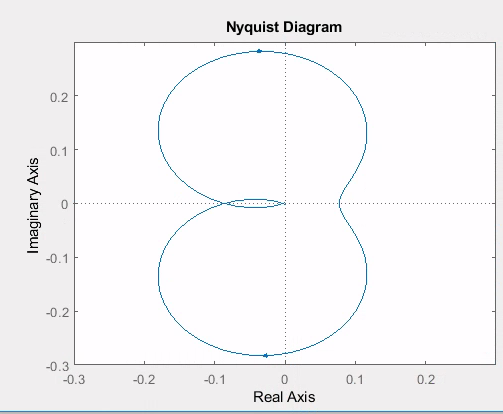
\includegraphics[width=0.5\linewidth]{nyquist215.png}
    \caption{Lieu de Nyquist}
    \label{fig:nyquist215}
\end{figure}
\subsection{}
On trace le diagramme de Bode pour le système :
\begin{figure}[h]
    \centering
    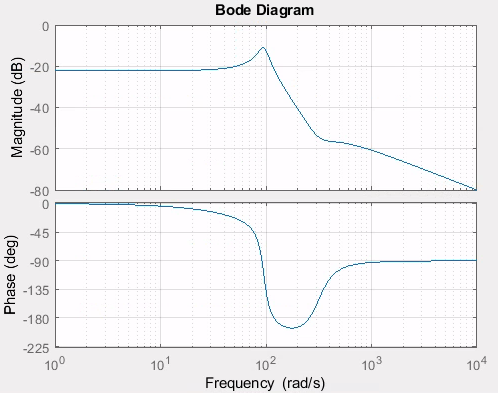
\includegraphics[width=0.5\linewidth]{bode217.png}
    \caption{Diagramme de Bode}
    \label{fig:bode217}
\end{figure}
\subsection{}
Afin d'obtenir une marge de phase de 45° il faut appliquer une correction de +12 dB. Soit :
\begin{align*}
    20\log(K_C)&=12\\
    K_C&=10^{12/20}\approx3.98
\end{align*}
On a vu que pour la précision, on devait avoir $K_C>135.8$, Or, on a vu que pour une marge de 45° on doit avoir $K_C=3.98$. Les deux conditions ne sont donc pas compatibles.
\subsection{}
En utilisant sisotool, on remarque qu'en prenant $K_C=608$, on a une marge de phase de 45° et on rentre dans toutes les conditions de stabilité et de précisions.
\subsection{}
Grâce à sisotool, on trouve la réponse indicielle suivante :
\begin{figure}[h]
    \centering
    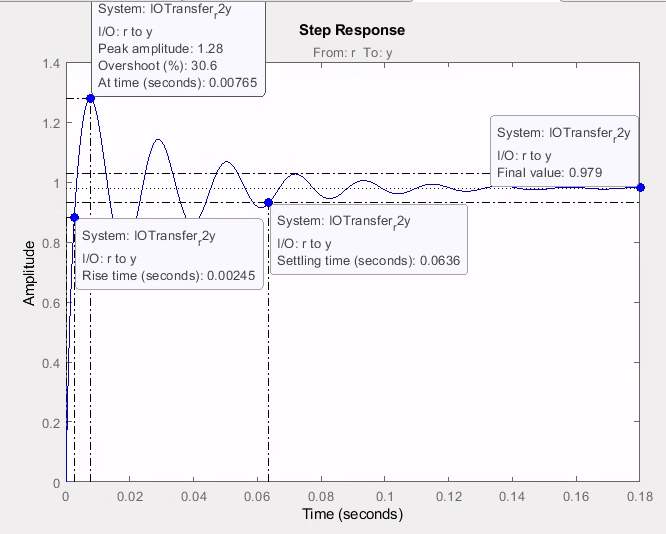
\includegraphics[width=0.75\linewidth]{sisotool2111.png}
    \caption{Réponse indicielle}
\end{figure}
\section{Correcteur PID}
\subsection{}
On choisit le correcteur à (correcteur PI).
Ce correcteur a pour expression :
\begin{align*}
    C(s)&=K_C\left(1+\frac{1}{T_Is}\right)=K_C+\frac{K_C}{T_Is}\\
    &=\frac{K_C(T_Is+1)}{T_Is}
\end{align*}
Ce correcteur admet comme pôle $p=0$ et comme zéro $z=-\frac{1}{T_I}$.
\end{document}
